\section{Zielsetzung}
\label{sec:Zielsetzung}
Diodenaser sind von zentraler Bedeutung in der Physik, da mit ihrem starken Output von kohärenten
Licht innerhalb eines schmalen Frequenzsprektrums sehr gut atomare Strukturen bzw. Quantensysteme
untersucht werden können. Außerdem können die Laser auf eine bestimmte Wellenlänge eingestellt werden, 
wodurch sie sich optimal auf das zu untersuchende System anpassen lassen.
In diesem Versuch soll die Funktionsweise eines Diodenlasers näher untersucht werden, indem die
Fluoreszenz von Rubidium nachgewiesen wird. Dafür müssen die verschiedenen Laserparamter so justiert werden,
dass die für Rubidium benötigte Wellenlänge erzeugt wird.

\section{Theorie}
\label{sec:Theorie}

\begin{figure}
    \centering
    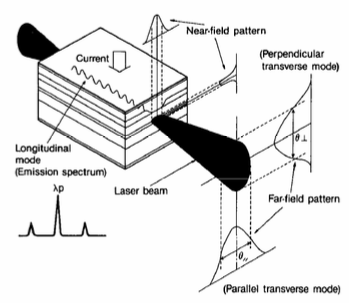
\includegraphics{content/pics/laser.png}
    \caption{Laserskizze. \cite{V60}}
    \label{fig:laser}
\end{figure}
